\section{Results}
Like in the methods section, this section will also be given in two parts. This is due to the two compression methods being so different in nature which means they cannot be directly compared. To compare the methods, a set of metrics will be applied to the original and compressed models respectively. The metrics include:
\begin{itemize}
    \item \textbf{Accuracy} - especially the accuracy drop is an important metric in comparing the compressed model to the full model, since there is trade-off between computational speed and accuracy
    \item \textbf{Number of Parameters} - how much space the model takes to store. This is important if small devices with limited storage space should be able to run the model
    \item \textbf{Theoretical speed} - based on the number of FLOPs, calculated using the formulas given in \autoref{tex:computational_complexity}. This is the actual number of calculations that is needed to perform a forward push. This should a good metric for the speed that can be calculated beforehand and used to predict the speed / speed-up of an algorithm.
    \item \textbf{Actual speed} - how long it takes to compute a forward push. Reported as the mean and standard deviation of many timings of the forward push. Due to potential differences in performance improvements, the methods will both be timed running on a CPU and GPU.
\end{itemize}
In the best case scenario, the actual speed improvement observed from timing the algorithms will be perfectly correlated with the calculated theoretical speed-up. Initially the results of method 1 will be given including observations from a small experiment, following this the results of applying method 2 will be given. Method 2 will also be applied to the well-known VGG-16 architecture\cite{Simonyan2015}, which have also been done by Kim et al.\cite{Kim2016}, however only on the convolutional layers.

\subsection{Method 1}
This is the method that decomposes the input into a NN. In order to get a better understanding of what happens when using this method, an experiment with only two classes for each data set and a rank of 2 will be carried out, and visual results will be given. Afterwards the results of using different ranks will be listed in order to assess performance differences.

\subsubsection{Experiment with low rank} \label{tex:result_experiment}
In the following an experiment is carried out to check whether the decomposition itself can carry much of the training. Since we have only 2 classes for the THETIS data set, and for the sake of the experiment 2 digits from the MNIST data set will be used. Since there are 2 classes in each data set, an initial rank of 2 will be experimentally chosen in the between sample dimension, since this also allows for a nice visualization of the loadings. The results for both the data set are described in the following.

\paragraph{Using MNIST 3s and 4s}
Only the MNIST observations depicting either a 3 or a 4 will be considered in this experiment. These digits are chosen due to their distinct shapes, hence ease of classification. Since the purpose is to make the algorithm find the differences between the two different digits, the spatial dimensions will not be decomposed. Using the experimental rank of 2, the decomposition of $N$ stacked 3s and 4s becomes:
\begin{equation}
    \tensor{X}^{N\times 28\times 28} \approx \tensor{G}^{2 \times 28 \times 28} \times_1 \bs{A}^{N\times 2} \qquad \Leftrightarrow \qquad \bs{X}_{(1)} \approx \bs{A}^{N\times 2} \ \bs{G}^{2 \times 28\cdot 28}_{(1)}
\end{equation}
Where $\bs{A}$ is the loading matrix in the dimension corresponding to different pictures. With the rank equal to 2, $\bs{A}$ holds 2 values per picture that should ideally be separating the two digits that is to be trained. \autoref{fig:decompExample3_4} shows how the decomposition of the first 100 training examples turns out. It seems the decomposition is able how to find the "general 3" and the "general 4", and then simply use the loadings of $\bs{A}$ to specify how much of each should be used to represent every observation. \autoref{fig:loadingAMatrix} shows a scatter-plot of the values of $\bs{A}$ colored to show the loadings corresponding to 3s and 4s respectively. There is some overlap between the two clusters, but it seems that they can be fairly distinguished. The mean of the loadings of the the 3s, 4s and overall respectively are also plotted in \autoref{fig:loadingAMatrix} and have been used to make the approximations shown in \autoref{fig:loadingsOfA}b-d. Here it is clear how an approximation is part 3, and part 4, and that the loadings specify how much.
\begin{figure}
    \centering
    \begin{subfigure}{0.45\linewidth}
        \centering
        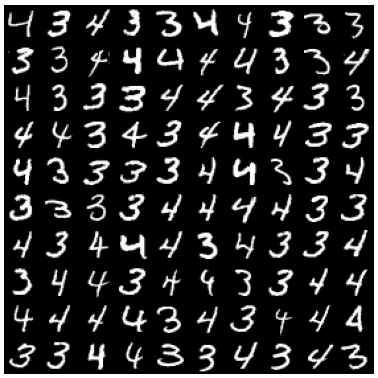
\includegraphics[width=\linewidth]{Pics/06_results/3_4_original.png}
        \captionsetup{width=.9\linewidth}
        \caption{Original MNIST training examples including only 3s and 4s.}
    \end{subfigure}
    \begin{subfigure}{0.45\linewidth}
        \centering
        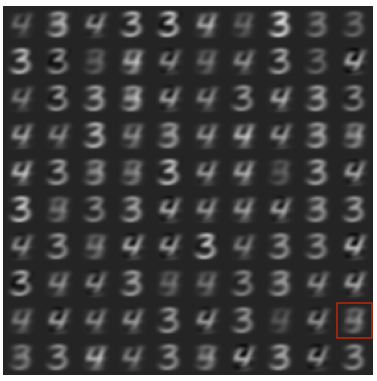
\includegraphics[width=\linewidth]{Pics/06_results/3_4_decomp.png}
        \captionsetup{width=.9\linewidth}
        \caption{Approximated versions of the training examples on the left, using the decomposition.}
    \end{subfigure}
    \captionsetup{width=.95\linewidth}
    \caption{MNIST training examples before and after decomposing with only rank 2 in the input dimension. Notice how the decomposed 3s and 4s look somehow standardized. It seems that every picture is a part standardized 3 and a part standardized 4. Notice how original digits that look relatively odd results in less certain approximation, e.g. the one highlighted with the red square.}
    \label{fig:decompExample3_4}
\end{figure}
\begin{figure}
    \centering
    \begin{subfigure}{0.99\linewidth}
        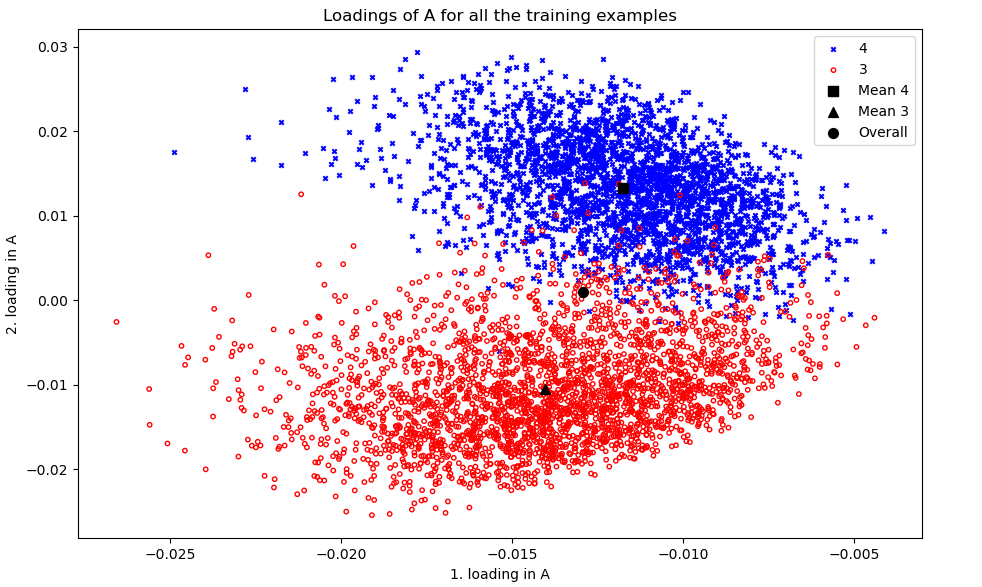
\includegraphics[width=\linewidth]{Pics/06_results/LoadingsOfAScatterMNIST.png}
        \caption{Scatter plot of the 2 loadings of the loading matrix $\bs{A}$ for the MNIST 3s and 4s respectively using rank 2 in the input dimension. The mean of the 2 clusters and overall is also marked with black.}
        \label{fig:loadingAMatrix}
    \end{subfigure}
    \begin{subfigure}{0.3\linewidth}
    \centering
        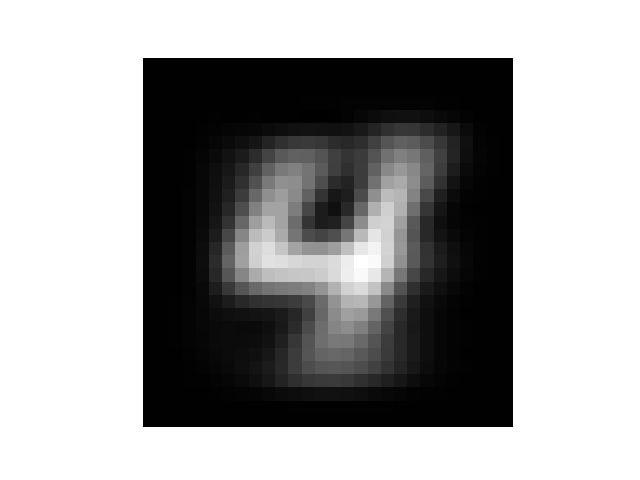
\includegraphics[width=.5\linewidth]{Pics/06_results/general4.png}
        \caption{The mean of 4s loadings}
    \end{subfigure}
    \begin{subfigure}{0.3\linewidth}
    \centering
        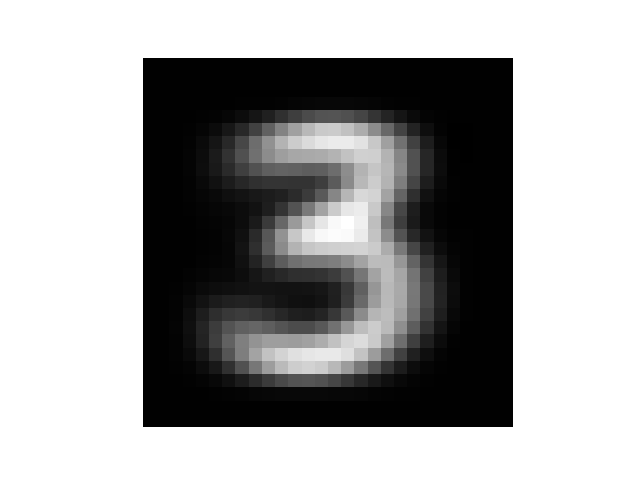
\includegraphics[width=.5\linewidth]{Pics/06_results/general3.png}
        \caption{The mean of 3s loadings}
    \end{subfigure}
    \begin{subfigure}{0.3\linewidth}
    \centering
        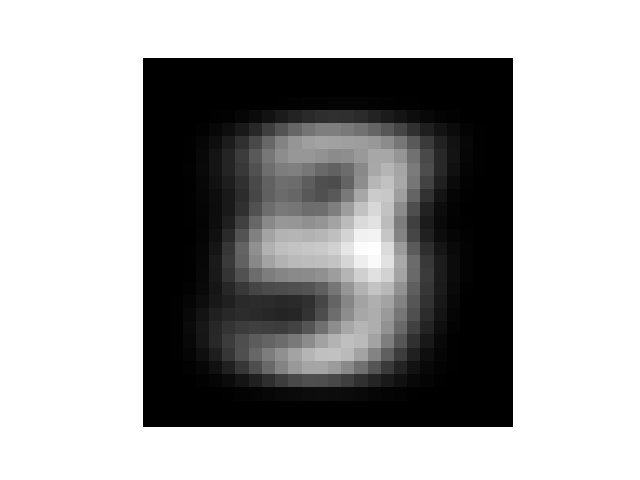
\includegraphics[width=.5\linewidth]{Pics/06_results/general.png}
        \caption{The mean of all loadings}
        \label{Hej}
    \end{subfigure}
    \caption{Scatter plot of the 2 loadings of $\bs{A}$ for the MNIST 3s and 4s using rank 2 including mean in each of the clusters and overall. Using these means as loadings in the approximation gives the approximated "general" 3, 4 and overall given in \textbf{(b)-(d)}. Notice how the overall mean gives a mixture of a 3 and a 4.}
    \label{fig:loadingsOfA}
\end{figure}

In the end this all comes down to the loadings of $\bs{A}$ holding a great deal of information about which pictures are 3s and which are 4s. This information could be used as input into the NN instead of the actual pictures, potentially reducing the number of parameters dramatically (from 784 to 2 input neurons in this example). Training the network with this input and only 1 hidden neuron in the ANN achieved a testing accuracy of $\approx 97 \%$, which is good compared to simply using all the pixel values as inputs which achieved a testing accuracy of $\approx 95\%$.

\paragraph{Using THETIS forehand flat and backhand}
Following the same procedure as for the MNIST 3s and 4s the rank of the decomposition is experimentally set to 2. Stacking $N$ videos and decomposing with rank 2 in the between sample dimension, and leaving the remaining dimensions uncompressed, yield:
\begin{equation}
    \tensor{X}^{N\times 4 \times 28 \times 120 \times 160} \approx \tensor{G}^{2 \times 4 \times 28 \times 120 \times 160} \times_1 \bs{A}^{N\times 2}
\end{equation}
Now the loading matrix $\bs{A}$ holds 2 values for each observation that should ideally be separating the two types of shots. Making the scatter plot of the loadings from $\bs{A}$ colored according to the type of shot shows that this is however not the case. The scatter plot is shown in \autoref{fig:scatter_plot_THETIS}, where it is clear that there are two clusters. The clusters however do not separate the type of shot, but instead the location of the video. This means that the location gives the decomposition algorithm more information about the video than the type of shot. The mean of each of the clusters have been used to approximate the videos from which the frames given in \autoref{fig:scatter_plot_THETIS}(b) and (c) are taken from.
\begin{figure}
    \centering
    \begin{subfigure}{\linewidth}
        \centering
        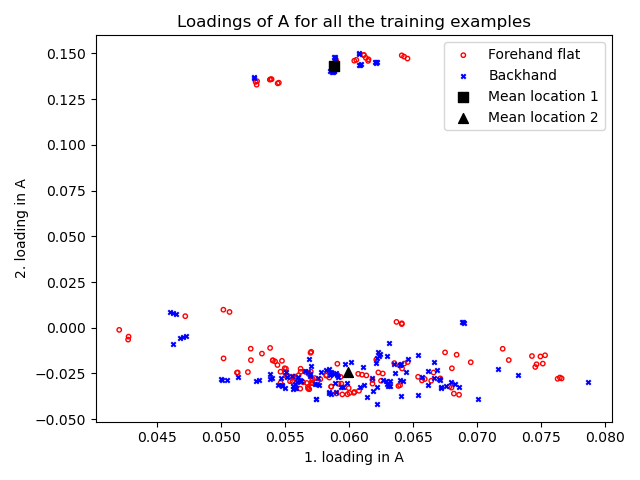
\includegraphics[width=0.64\linewidth]{Pics/06_results/scatter_loadings_THETIS.png}
        \captionsetup{width=.95\linewidth}
        \caption{Scatter plot of the loadings of $\bs{A}$ for the THETIS forehands and backhands. There seems to be two clusters, but they are not divided according to the shot type, but rather the background information. The mean of the two clusters that are given, have been used to approximate the videos in \textbf{(b)} and \textbf{(c)}.}
    \end{subfigure}
    \begin{subfigure}{.4\linewidth}
        \centering
        \captionsetup{width=.95\linewidth}
        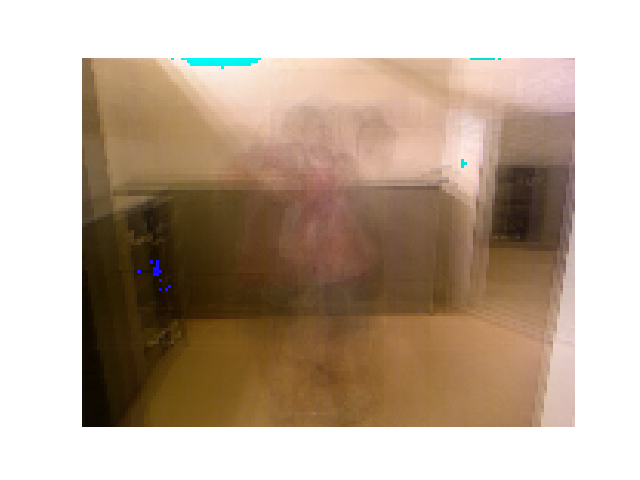
\includegraphics[width=\linewidth]{Pics/06_results/loc1.png}
        \caption{Approximation using the loadings of the mean of the little (top) cluster in \textbf{(a)}. This corresponds to one of the two locations (changing room).}
    \end{subfigure}
    \begin{subfigure}{.4\linewidth}
        \centering
        \captionsetup{width=.95\linewidth}
        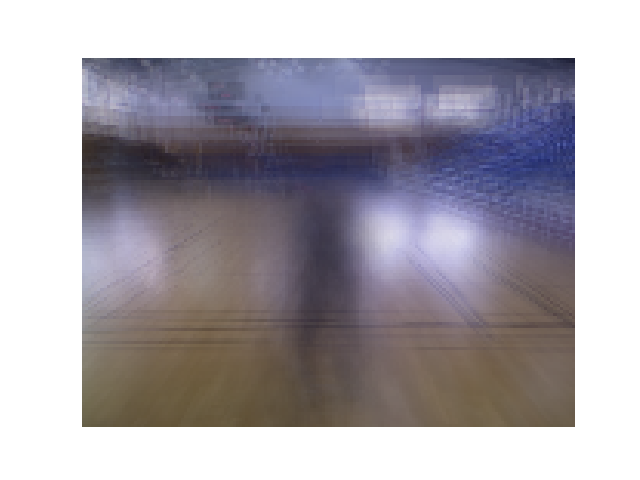
\includegraphics[width=\linewidth]{Pics/06_results/loc2.png}
        \caption{Approximation using the loadings of the mean of the big (bottom) cluster in \textbf{(a)}. This corresponds to one of the two locations (indoor arena).}
    \end{subfigure}
    \begin{subfigure}{.4\linewidth}
        \centering
        \captionsetup{width=.95\linewidth}
        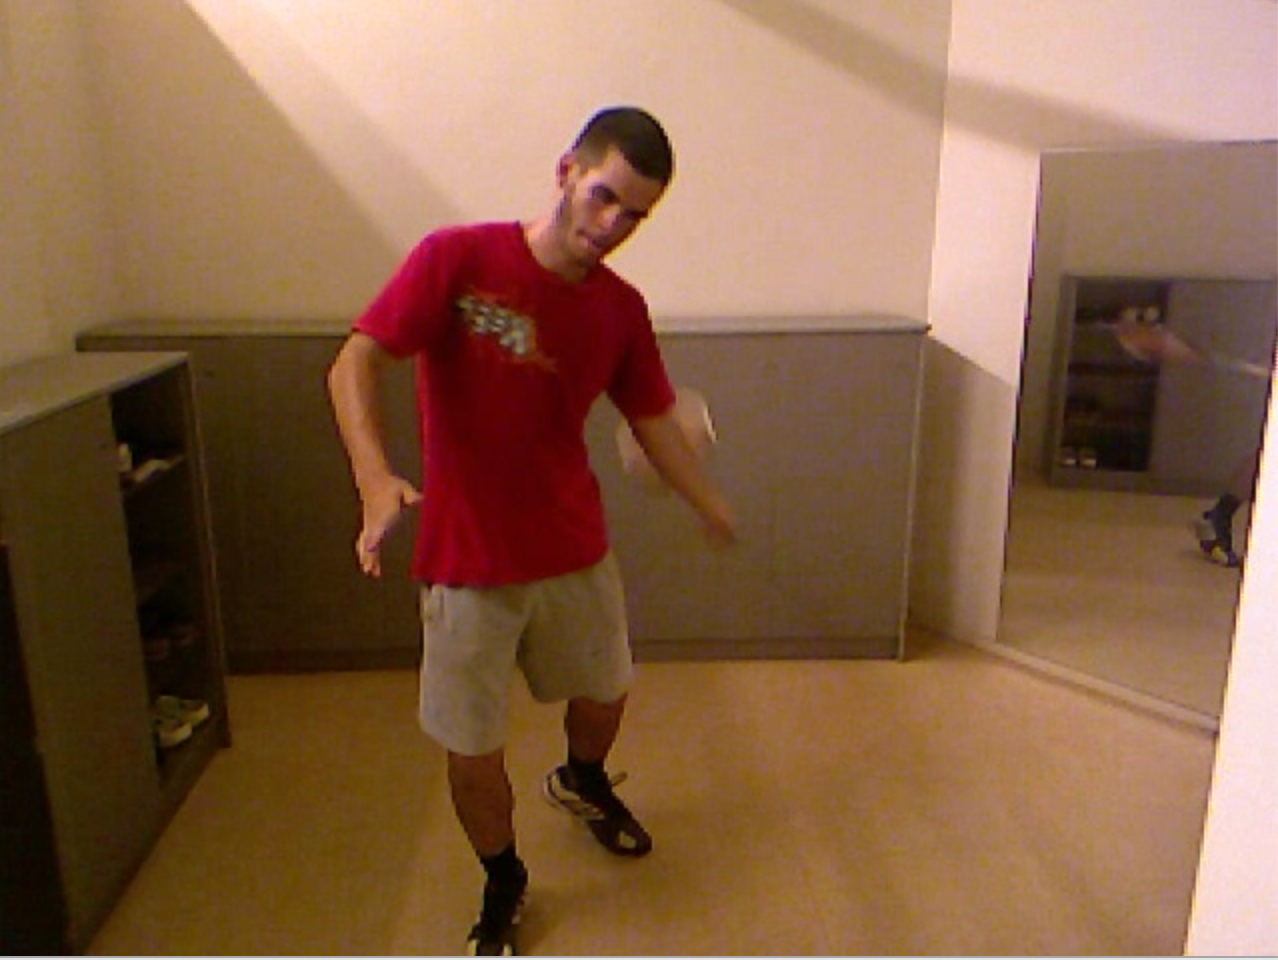
\includegraphics[width=.78\linewidth]{Pics/06_results/loc_1_real.png}
        \caption{An example of the changing room seen approximated in \textbf{(b)}}
    \end{subfigure}
    \begin{subfigure}{.4\linewidth}
        \centering
        \captionsetup{width=.95\linewidth}
        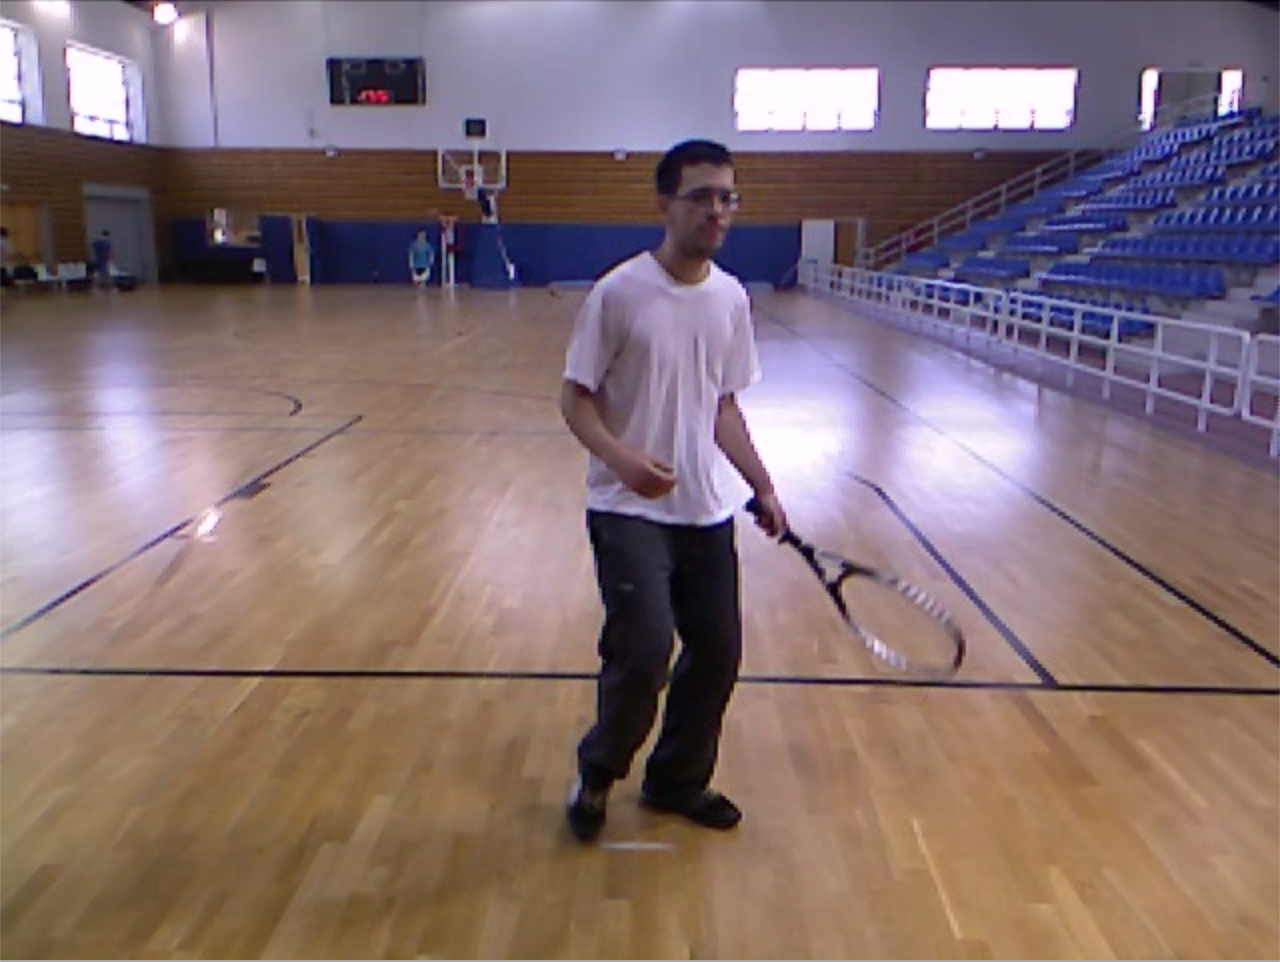
\includegraphics[width=.78\linewidth]{Pics/06_results/loc_2_real.png}
        \caption{An example of the indoor arena seen approximated in \textbf{(c)}}
    \end{subfigure}
    \caption{The loadings of $\bs{A}$ for the THETIS data illustrated by a scatter plot in \textbf{(a)}, and used to make the two approximation \textbf{(b)} and \textbf{(c)} by estimating the mean of each cluster seen in the scatter plot. It is clear how the two clusters in \textbf{(a)} separates the two locations, instead of the type of shot}
    \label{fig:scatter_plot_THETIS}
\end{figure}
This means that even though all the temporal information is given to the algorithm, the background is still the thing that separates the videos more. In order to differentiate the different type of shots more needs to be done as, e.g. increasing the rank allowing the algorithm to look for finer details or using some algorithm to remove the background. The accuracies after training this model are very low and not higher than a random classification.

\subsubsection{Results for MNIST}
The results for MNIST using the method that decomposes the input are given in \autoref{tab:res_input_MNIST}. Here the different models have been trained and timed, reporting the mean and the standard deviation of the time of 1,000 forward pushes through the network, assuming the core $\tensor{G}$ have already been matricized and inverted in \eqref{eq:estimation_of_loading_A}. Since the data is small and the models are all very fast, every forward push is conducted using 10 observations, which means that a total of 10,000 forward pushes have been timed. In \autoref{tab:res_input_MNIST}
the brackets holds the time of each of the two parts of the algorithm, i.e. estimating the input loadings ($\bs{A}$), and pushing these through the ANN. 

It seems that the compressed model exceeds the number of parameters and FLOPs of the full input model at the rank of around 20 where the accuracy is significantly lower than that of the original. Considering the timing on the CPU - the compressed model exceeds the full input model even earlier (at around 10-11). This all questions the applicability of the method - at least for very simple problems. The time using the GPU is rather constant, since the GPU is so fast, that a relatively small change in the number of calculations will not result in a big difference in the computation time. Actually the full input network is faster on the GPU than every one of the compressed models, meaning that the penalty of having multiple steps to the algorithm is too big.
\begin{table}
\small
\centering
\captionsetup{width=.95\linewidth}
\caption{The results of running the input decomposition method on the MNIST data set using different ranks for the decomposition. The time is reported as the mean and standard deviation of 1,000 samples where 10 observations are evaluated using the model. The ratios are calculated between the attributes of the given compressed model and the model in which the full input is simply given to the ANN. The accuracy seems to increase with along with the rank. Notice however that even though the rank of the decomposition is very high, the accuracy of the full input network is not reached - not even using 7.6 times the FLOPs (rank 150)}
\label{tab:res_input_MNIST}
\begin{tabular}{c|cccc|c}
\textbf{Rank}     & \textbf{\begin{tabular}[c]{@{}c@{}}Parameters\\ (K)\end{tabular}} & \textbf{\begin{tabular}[c]{@{}c@{}}FLOPs\\ (K)\end{tabular}} & \textbf{\begin{tabular}[c]{@{}c@{}}Time CPU\\ (ms)\end{tabular}}                  & \textbf{\begin{tabular}[c]{@{}c@{}}Time GPU\\ (ms)\end{tabular}}                  & \textbf{\begin{tabular}[c]{@{}c@{}}Accuracy\\ (\%)\end{tabular}} \\ \hline
\textbf{2}        & 1.83                                                              & 3.58                                                         & \begin{tabular}[c]{@{}c@{}}$1.481 \pm 0.025$ \\ $(= 0.904 + 0.647 )$\end{tabular} & \begin{tabular}[c]{@{}c@{}}$0.149 \pm 0.012$ \\ $(= 0.014 + 0.118 )$\end{tabular} & \textbf{33.61}                                                  \\
ratio             & 0.11                                                              & 0.11                                                         & 0.871                                                                             & 1.155                                                                             & 0.36                                                            \\ \hline
\textbf{5}        & 4.25                                                              & 8.41                                                         & \begin{tabular}[c]{@{}c@{}}$2.445 \pm 0.039$\\  $(= 1.885 + 0.551 )$\end{tabular} & \begin{tabular}[c]{@{}c@{}}$0.144 \pm 0.011$\\  $(= 0.013 + 0.115 )$\end{tabular} & \textbf{52.20}                                                  \\
ratio             & 0.25                                                              & 0.26                                                         & 1.438                                                                             & 1.116                                                                             & 0.55                                                            \\ \hline
\textbf{7}        & 5.86                                                              & 11.62                                                        & \begin{tabular}[c]{@{}c@{}}$3.114 \pm 0.047$ \\ $(= 2.525 + 0.565 )$\end{tabular} & \begin{tabular}[c]{@{}c@{}}$0.142 \pm 0.010$\\  $(= 0.013 + 0.113 )$\end{tabular} & \textbf{61.71}                                                  \\
ratio             & 0.35                                                              & 0.37                                                         & 1.832                                                                             & 1.101                                                                             & 0.65                                                            \\ \hline
\textbf{10}       & 8.27                                                              & 16.44                                                        & \begin{tabular}[c]{@{}c@{}}$1.660 \pm 0.033$\\  $(= 0.968 + 0.681 )$\end{tabular} & \begin{tabular}[c]{@{}c@{}}$0.141 \pm 0.011$\\  $(= 0.013 + 0.113 )$\end{tabular} & \textbf{67.55}                                                  \\
ratio             & 0.50                                                              & 0.52                                                         & 0.976                                                                             & 1.093                                                                             & 0.72                                                            \\ \hline
\textbf{15}       & 12.30                                                             & 24.48                                                        & \begin{tabular}[c]{@{}c@{}}$1.906 \pm 0.035$ \\ $(= 1.372 + 0.527 )$\end{tabular} & \begin{tabular}[c]{@{}c@{}}$0.141 \pm 0.011$\\  $(= 0.013 + 0.113 )$\end{tabular} & \textbf{72.14}                                                  \\
ratio             & 0.74                                                              & 0.77                                                         & 1.121                                                                             & 1.093                                                                             & 0.76                                                            \\ \hline
\textbf{20}       & 16.32                                                             & 32.51                                                        & \begin{tabular}[c]{@{}c@{}}$1.965 \pm 0.031$\\  $(= 1.354 + 0.598 )$\end{tabular} & \begin{tabular}[c]{@{}c@{}}$0.142 \pm 0.011$\\  $(= 0.014 + 0.113 )$\end{tabular} & \textbf{79.41}                                                  \\
ratio             & 0.98                                                              & 1.02                                                         & 1.156                                                                             & 1.101                                                                             & 0.84                  \\ \hline
\textbf{30}       & 24.37                                                             & 48.58                                                        & \begin{tabular}[c]{@{}c@{}}$2.397 \pm 0.035$ \\ $(= 1.785 + 0.599 )$\end{tabular} & \begin{tabular}[c]{@{}c@{}}$0.142 \pm 0.011$\\  $(= 0.015 + 0.115 )$\end{tabular} & \textbf{74.66}                                                  \\
ratio             & 1.46                                                              & 1.53                                                         & 1.410                                                                             & 1.101                                                                             & 0.79                                                            \\ \hline
\textbf{40}       & 32.42                                                             & 64.65                                                        & \begin{tabular}[c]{@{}c@{}}$2.298 \pm 0.039$ \\ $(= 1.756 + 0.528 )$\end{tabular} & \begin{tabular}[c]{@{}c@{}}$0.144 \pm 0.011$ \\ $(= 0.024 + 0.116 )$\end{tabular} & \textbf{74.89}                                                  \\
ratio             & 1.94                                                              & 2.04                                                         & 1.352                                                                             & 1.116                                                                             & 0.79                                                            \\ \hline
\textbf{50}       & 40.47                                                             & 80.72                                                        & \begin{tabular}[c]{@{}c@{}}$3.005 \pm 0.043$\\  $(= 2.242 + 0.752 )$\end{tabular} & \begin{tabular}[c]{@{}c@{}}$0.146 \pm 0.013$\\  $(= 0.025 + 0.114 )$\end{tabular} & \textbf{81.56}                                                  \\
ratio             & 2.43                                                              & 2.54                                                         & 1.768                                                                             & 1.132                                                                             & 0.86                                                            \\ \hline
\textbf{70}       & 56.57                                                             & 112.86                                                       & \begin{tabular}[c]{@{}c@{}}$3.661 \pm 0.047$\\  $(= 3.042 + 0.581 )$\end{tabular} & \begin{tabular}[c]{@{}c@{}}$0.144 \pm 0.010$ \\ $(= 0.022 + 0.115 )$\end{tabular} & \textbf{75.13}                                                  \\
ratio             & 3.39                                                              & 3.56                                                         & 2.154                                                                             & 1.116                                                                             & 0.80                                                            \\ \hline
\textbf{100}      & 80.72                                                             & 161.07                                                       & \begin{tabular}[c]{@{}c@{}}$4.796 \pm 0.067$ \\ $(= 3.897 + 0.823 )$\end{tabular} & \begin{tabular}[c]{@{}c@{}}$0.144 \pm 0.011$ \\ $(= 0.027 + 0.114 )$\end{tabular} & \textbf{83.98}                                                  \\
ratio             & 4.84                                                              & 5.08                                                         & 2.821                                                                             & 1.116                                                                             & 0.89                                                            \\ \hline
\textbf{150}      & 120.97                                                            & 241.42                                                       & \begin{tabular}[c]{@{}c@{}}$6.664 \pm 0.086$\\  $(= 5.655 + 0.849 )$\end{tabular} & \begin{tabular}[c]{@{}c@{}}$0.145 \pm 0.012$\\  $(= 0.034 + 0.115 )$\end{tabular} & \textbf{83.65}                                                  \\
ratio             & 7.25                                                              & 7.61                                                         & 3.920                                                                             & 1.124                                                                             & 0.89                                                            \\ \hline
\textbf{Full input} & 16.68                                                             & 31.73                                                        & $1.700 \pm 0.052 $                                                                & $0.129 \pm   0.013$                                                               & \textbf{94.44}                                                 
\end{tabular}
\end{table}

\subsubsection{Results for THETIS}
The results for THETIS are given in \autoref{tab:res_input_THETIS}. The time is given as the mean and standard deviation of the time based on 1,000 forward pushes through the different models, assuming the core $\tensor{G}$ have already been matricized and inverted in \eqref{eq:estimation_of_loading_A}. The brackets holds the time broken down into the two parts - estimating the loading matrix and pushing through the ANN.

Interestingly the accuracy of the decomposed model actually exceed that of the full input model when the rank is chosen big (150). Unfortunately the computational complexity and the computation time are both exceeded at this point. The compressed model exceed the computational complexity and time (CPU) at a rank around 100, where the accuracy does not match that of the full input model. This fact casts doubt on the functionality of this method. When running on the GPU the computation time is exceeded at an even lower rank, which could be due to the GPU being more penalized by the split into two steps as was also noted for the MNIST data set. 

Another thing to notice is that the estimation of the loading matrix accounts for the majority of the computation time by far. This is due to the estimation of the loadings being a rather big matrix-matrix product, since it gets the full input ($>2$ M values).
\begin{table}
\centering
\caption{Results for running the input decomposition algorithm on the THETIS data set using different ranks for the decomposition. The time is given as the mean and standard deviation of 1,000 forward pushed for each model. The numbers in brackets correspond to the break-down of the time of the estimation of the input loadings ($\bs{A}$) and the forward push through the network. The ratios are calculated between the attributes of the given compressed model and the model simply using the full input into the given ANN. Notice how the accuracy of the original network is not reached before reaching rank 150, exceeding the complexity and time by around 50 \% (73\% for GPU)}
\label{tab:res_input_THETIS}
\small
\begin{tabular}{c|cccc|c}
\textbf{Rank}     & \textbf{\begin{tabular}[c]{@{}c@{}}Parameters\\ (M)\end{tabular}} & \textbf{\begin{tabular}[c]{@{}c@{}}FLOPs \\ (M)\end{tabular}} & \textbf{\begin{tabular}[c]{@{}c@{}}Time CPU \\ (ms)\end{tabular}}                     & \textbf{\begin{tabular}[c]{@{}c@{}}Time GPU \\ (ms)\end{tabular}}                 & \textbf{\begin{tabular}[c]{@{}c@{}}Accuracy \\ (\%)\end{tabular}} \\ \hline
\textbf{30}       & 64.52                                                             & 129.03                                                        & \begin{tabular}[c]{@{}c@{}}$30.534 \pm 0.325$ \\ $(= 30.322 + 0.081 )$\end{tabular}   & \begin{tabular}[c]{@{}c@{}}$0.340 \pm 0.073$ \\ $(= 0.246 + 0.209 )$\end{tabular} & \textbf{70}                                                      \\
ratio             & 0.30                                                              & 0.30                                                          & 0.33                                                                                  & 0.33                                                                              & 0.76                                                             \\ \hline
\textbf{40}       & 86.02                                                             & 172.04                                                        & \begin{tabular}[c]{@{}c@{}}$38.481 \pm 0.371$\\  $(= 38.085 + 0.087 )$\end{tabular}   & \begin{tabular}[c]{@{}c@{}}$0.496 \pm 0.102$\\  $(= 0.357 + 0.243 )$\end{tabular} & \textbf{70}                                                      \\
ratio             & 0.40                                                              & 0.40                                                          & 0.42                                                                                  & 0.47                                                                              & 0.76                                                             \\ \hline
\textbf{50}       & 107.53                                                            & 215.05                                                        & \begin{tabular}[c]{@{}c@{}}$47.790 \pm 0.300$ \\ $(= 47.474 + 0.093 )$\end{tabular}   & \begin{tabular}[c]{@{}c@{}}$0.685 \pm 0.155$ \\ $(= 0.491 + 0.285 )$\end{tabular} & \textbf{82}                                                      \\
ratio             & 0.50                                                              & 0.50                                                          & 0.52                                                                                  & 0.66                                                                              & 0.89                                                             \\ \hline
\textbf{60}       & 129.03                                                            & 258.06                                                        & \begin{tabular}[c]{@{}c@{}}$58.151 \pm 0.373$\\  $(= 57.811 + 0.093 )$\end{tabular}   & \begin{tabular}[c]{@{}c@{}}$0.729 \pm 0.149$ \\ $(= 0.521 + 0.293 )$\end{tabular} & \textbf{78}                                                      \\
ratio             & 0.59                                                              & 0.60                                                          & 0.63                                                                                  & 0.70                                                                              & 0.85                                                             \\ \hline
\textbf{70}       & 150.54                                                            & 301.07                                                        & \begin{tabular}[c]{@{}c@{}}$72.011 \pm 0.450$ \\ $(= 71.641 + 0.092 )$\end{tabular}   & \begin{tabular}[c]{@{}c@{}}$0.940 \pm 0.186$ \\ $(= 0.674 + 0.340 )$\end{tabular} & \textbf{74}                                                      \\
ratio             & 0.69                                                              & 0.70                                                          & 0.76                                                                                  & 0.90                                                                              & 0.80                                                             \\ \hline
\textbf{80}       & 172.04                                                            & 344.08                                                        & \begin{tabular}[c]{@{}c@{}}$75.648 \pm 0.398$ \\ $(= 75.409 + 0.093 )$\end{tabular}   & \begin{tabular}[c]{@{}c@{}}$0.793 \pm 0.159$ \\ $(= 0.568 + 0.308 )$\end{tabular} & \textbf{76}                                                      \\
ratio             & 0.79                                                              & 0.80                                                          & 0.82                                                                                  & 0.76                                                                              & 0.83                                                             \\ \hline
\textbf{90}       & 193.55                                                            & 387.09                                                        & \begin{tabular}[c]{@{}c@{}}$90.569 \pm 0.476$ \\ $(= 90.355 + 0.093 )$\end{tabular}   & \begin{tabular}[c]{@{}c@{}}$1.194 \pm 0.231$ \\ $(= 0.853 + 0.394 )$\end{tabular} & \textbf{82}                                                      \\
ratio             & 0.89                                                              & 0.90                                                          & 0.98                                                                                  & 1.14                                                                              & 0.89                                                             \\ \hline
\textbf{100}      & 215.05                                                            & 430.10                                                        & \begin{tabular}[c]{@{}c@{}}$99.905 \pm 0.591$ \\ $(= 99.507 + 0.093 )$\end{tabular}   & \begin{tabular}[c]{@{}c@{}}$1.346 \pm 0.257$\\  $(= 0.960 + 0.427 )$\end{tabular} & \textbf{82}                                                      \\
ratio             & 0.99                                                              & 1.00                                                          & 1.08                                                                                  & 1.29                                                                              & 0.89                                                             \\ \hline
\textbf{110}      & 236.56                                                            & 473.11                                                        & \begin{tabular}[c]{@{}c@{}}$106.205 \pm 0.685$ \\ $(= 106.114 + 0.092 )$\end{tabular} & \begin{tabular}[c]{@{}c@{}}$1.496 \pm 0.284$ \\ $(= 1.067 + 0.460 )$\end{tabular} & \textbf{80}                                                      \\
ratio             & 1.09                                                              & 1.10                                                          & 1.15                                                                                  & 1.43                                                                              & 0.87                                                             \\ \hline
\textbf{120}      & 258.06                                                            & 516.12                                                        & \begin{tabular}[c]{@{}c@{}}$113.461 \pm 0.986$ \\ $(= 113.081 + 0.093 )$\end{tabular} & \begin{tabular}[c]{@{}c@{}}$1.394 \pm 0.269$ \\ $(= 0.995 + 0.438 )$\end{tabular} & \textbf{88}                                                      \\
ratio             & 1.19                                                              & 1.20                                                          & 1.23                                                                                  & 1.33                                                                              & 0.96                                                             \\ \hline
\textbf{150}      & 322.58                                                            & 645.15                                                        & \begin{tabular}[c]{@{}c@{}}$138.881 \pm 0.910$ \\ $(= 138.528 + 0.094 )$\end{tabular} & \begin{tabular}[c]{@{}c@{}}$1.809 \pm 0.339$\\  $(= 1.288 + 0.528 )$\end{tabular} & \textbf{94}                                                      \\
ratio             & 1.49                                                              & 1.50                                                          & 1.51                                                                                  & 1.73                                                                              & 1.02                                                             \\ \hline
\textbf{200}      & 430.10                                                            & 860.20                                                        & \begin{tabular}[c]{@{}c@{}}$174.968 \pm 1.870$\\  $(= 174.853 + 0.094 )$\end{tabular} & \begin{tabular}[c]{@{}c@{}}$2.362 \pm 0.429$ \\ $(= 1.682 + 0.648 )$\end{tabular} & \textbf{94}                                                      \\
ratio             & 1.98                                                              & 2.00                                                          & 1.90                                                                                  & 2.26                                                                              & 1.02                                                             \\ \hline
\textbf{Full input} & 217.19                                                            & 430.08                                                        & $ 95.243\pm 1.642 $                                                                   & $1.045 \pm 0.255 $                                                                & \textbf{92}                                                     
\end{tabular}
\end{table}

%%%%%%%%%%%%%%%%%%%%%%%%%%%%%%%%%%%%%%%%%%%%%%%%%%%%%%%%%%%%%%%%%%%%%%%%%%%%%%%%%%%%    
%%        Decomposing Pre-Trained Network    %%%%%%%%%%%%%%%%%%%%%%%%%%%%%%%%%%%%%%%
%%%%%%%%%%%%%%%%%%%%%%%%%%%%%%%%%%%%%%%%%%%%%%%%%%%%%%%%%%%%%%%%%%%%%%%%%%%%%%%%%%%%


\subsection{Method 2}
This method is the one compressing a pre-trained network. Since the rank selection is a part of the method itself as described in \autoref{tex:rank_selection}, there will be no results for different ranks, but simply the ranks given by the algorithm. The results will however be given by layer which means that the effect of the compression on different types and sizes of layers can be assessed. The results using the architectures of the two data sets will be given individually in the following including accuracies of the original network and the compressed network before and after fine-tuning. Lastly, the results of applying method 2 to the VGG-16 architecture will be given, though without reporting accuracy.

\subsubsection{Results for MNIST}
After having run method 2 on the MNIST architecture given in \autoref{fig:architecture_choices}, the ranks of the decomposition along with the theoretical speed-ups and storage improvements are given in \autoref{tab:res_MNIST_FLOPs}. An overview of the compressed network is given in \autoref{tab:res_MNIST_dcmp_architecture}. The arrows bind together two layers in a sequence
\begin{table}
\centering
\captionsetup{width=.95\linewidth}
\caption{The resulting compressed network after applying method 2 to the MNIST architecture given in \autoref{fig:architecture_choices}. Every bracket is a layer in the network. The convolutions are expressed as (in channels, out channels, [kernel size]). The linear layers are expressed as (in neurons, out neurons)}
\label{tab:res_MNIST_dcmp_architecture}
\begin{tabular}{cll}
\textbf{Layer}            & \textbf{Original}              & \textbf{Compressed}                                                          \\ \hline
Conv 1                    & (1, 6, [5, 5])                 & (1, 1, [5, 5]) $\rightarrow$ (1, 6, [1, 1])                                  \\
Conv 2                    & (6, 16, [5, 5])                & $ (6, 4, [1, 1]) \rightarrow (4, 6, [5, 5]) \rightarrow (6, 16, [1, 1]) $    \\ \hline
\multicolumn{1}{l}{Lin 1} & \multicolumn{1}{l}{(400, 120)} & \multicolumn{1}{l}{$ (400, 18) \rightarrow (18, 18) \rightarrow (18, 120) $} \\
\multicolumn{1}{l}{Lin 2} & \multicolumn{1}{l}{(120, 84)}  & \multicolumn{1}{l}{$ (120, 9) \rightarrow (9, 84) $}                        
\end{tabular}
\end{table}
The accuracies of the original and compressed networks are given here:
\begin{table}[H]
\centering
\begin{tabular}{cccl}
\textbf{Original} & \multicolumn{2}{c}{\textbf{Compressed}} & \textbf{Drop} \\
                  & Before fine-tuning  & After fine-tuning &               \\
98.66 \%          & 66.12 \%            & 98.19 \%          & -0.47 \%        
\end{tabular}
\end{table}
Here the accuracy lost after compressing was quickly restored, and the accuracy drop is insignificant. The observed speed-up measured by timing the network is given layer-wise in \autoref{tab:res_MNIST_time}. Here the time is computed as the mean and standard deviation of 1,000 forward pushes of each 100 observations for both the CPU and GPU. The brackets hold the time for each of the sub-layers that the original layer is compressed into. The improvements are given as the ratio between the attribute of the original network and the attribute of the given layer.
\begin{table}
\centering
\small
\caption{Overview of the layers of the decomposed network resulting after applying method 2 to the MNIST architecture given in \autoref{tex:architectures} including number of weights and FLOPs for each layer. The number of FLOPs have been used to calculate the theoretical speed up, and the weights have been used to calculate the storage improvement. These results make method 2 look promising with an overall theoretical speed up of 3.45 times and an overall storage improvement of 4.62 times for the MNIST architecture}
\label{tab:res_MNIST_FLOPs}
\begin{tabular}{cc|cccc}
\multicolumn{2}{c}{\textbf{MNIST Layer}} & $ S / R_{in}$ & $ T /R_{out}$ & Weights         & FLOPs (K)                  \\ \specialrule{0.1em}{.05em}{.05em}
\multirow{3}{*}{Conv 1}  & Orig          & 1             & 6             & 156             & 231.28                     \\
                         & Comp          &               & 1             & 37              & 43.9 $(=38.42+5.49)$       \\
                         & \textit{Impr} &               &               & $ \times 4.22$  & $\times 5.27$              \\ \hline
\multirow{3}{*}{Conv 2}  & Orig          & 6             & 16            & 2416            & 478.5                      \\
                         & Comp          & 4             & 6             & 736             & 171.6 $(=34.5+119.4+17.7)$ \\
                         & \textit{Impr} &               &               & $ \times 3.28$  & $\times 2.79$              \\ \hline
\multirow{3}{*}{Lin 1}   & Orig          & 400           & 120           & 48120           & 96                         \\
                         & Comp          & 18            & 18            & 9804            & 19.33 $(=14.38+0.63+4.32)$ \\
                         & \textit{Impr} &               &               & $ \times 4.91$  & $\times 4.97$              \\ \hline
\multirow{3}{*}{Lin 2}   & Orig          & 120           & 84            & 10164           & 20.16                      \\
                         & Comp          & -             & 9             & 1920            & 3.66 $(=2.15+1.51)$        \\
                         & \textit{Impr} &               &               & $ \times 5.29$  & $\times 5.51$              \\ \hline
\multirow{3}{*}{Lin 3}     & Orig          & 84            & 10            & 850             & 1.68                       \\
                         & Comp          & -             & -             & 850             & 1.68                       \\
                         & \textit{Impr} & \textit{}     & \textit{}     & $ \times 1$     & $ \times 1.00$             \\ \specialrule{0.1em}{.05em}{.05em} 
\multirow{3}{*}{Total}   & Orig          &               &               & 61706           & 827.62                     \\
                         & Comp          &               &               & 13347           & 240.18                     \\
                         & \textit{Impr} &               &               & $ \times 4.62 $ & $\times 3.45 $            
\end{tabular}
\end{table}
\begin{table}
\centering
\small
\captionsetup{width=.9\linewidth}
\caption{Resulting observed speed-ups after applying method 2 to the MNIST architecture described in \autoref{fig:architecture_choices}. The time is reported as the mean and standard deviation of 1,000 forward pushes of each 100 observations. The brackets hold the time for each of the sub-layers the original layer is compressed into. The improvement is calculated as the ratio between the time of the original model and the time of the decomposed model, and $\times x$ means a speed-up of $x$ times. In this case the decomposed model does not do well. In every layer it is slower than the original layer, which results in a total speed-up of 0.57 (0.58) which means that it takes almost twice the time. Notice how the $1\times 1$ convolutions in Conv 2 both take more time than the middle convolution even though they use only 10\% and 20\% of the FLOPs respectively. There seem to be no significant differences between the speed-up using the CPU or GPU respectively}
\label{tab:res_MNIST_time}
\begin{tabular}{cc|cc}
\multicolumn{2}{c|}{\multirow{2}{*}{\textbf{MNIST Layer}}} & \multicolumn{2}{c}{\textbf{Time for 100 forward pushes (ms)}}         \\
\multicolumn{2}{c|}{}                                      & CPU                    & GPU                                  \\ \specialrule{0.1em}{.05em}{.05em}
\multirow{4}{*}{Conv 1}      & Orig                       & $7.085\pm 1.347$       & $0.143\pm 0.003$                     \\
                             & \multirow{2}{*}{Comp}      & $12.274\pm 0.207$      & $0.223\pm 0.003$                     \\
                             &                            & $(=3.422+8.852)$       & $(=0.087+0.136)$                     \\
                             & \textit{Impr}              & $ \times 0.577$        & $ \times 0.64$                       \\ \hline
\multirow{4}{*}{Conv 2}      & Orig                       & $2.279\pm 0.074$       & $0.156\pm 0.004$                     \\
                             & \multirow{2}{*}{Comp}      & $4.182\pm 0.104$       & $0.292\pm 0.004$                     \\
                             &                            & $(=1.401+0.876+1.906)$ & $(=0.074+0.089+0.128)$               \\
                             & \textit{Impr}              & $ \times 0.545$        & $ \times 0.54$                       \\ \hline
\multirow{4}{*}{Lin 1}       & Orig                       & $0.31\pm 0.067$        & $0.096\pm 0.002$                     \\
                             & \multirow{2}{*}{Comp}      & $0.373\pm 0.012$       & $0.235\pm 0.005$                     \\
                             &                            & $(=0.203+0.057+0.113)$ & $(=0.093+0.063+0.079)$               \\
                             & \textit{Impr}              & $ \times 0.831$        & $ \times 0.41$                       \\ \hline
\multirow{4}{*}{Lin 2}       & Orig                       & $0.11\pm 0.014$        & $0.078\pm 0.002$                     \\
                             & \multirow{2}{*}{Comp}      & $0.132\pm 0.006$       & $0.135\pm 0.004$                     \\
                             &                            & $(=0.057+0.075)$       & \multicolumn{1}{l}{$(=0.061+0.074)$} \\
                             & \textit{Impr}              & $ \times 0.833$        & $ \times 0.58$                       \\ \hline
\multirow{4}{*}{Lin 3}       & Orig                       & $0.112\pm 0.006$       & $0.08\pm 0.003$                      \\
                             & \multirow{2}{*}{Comp}      & $0.105\pm 0.004$       & $0.079\pm 0.001$                     \\
                             &                            &                        &                                      \\
                             & \textit{Impr}              & $ \times 1.067$        & $ \times 1.01$                       \\ \specialrule{0.1em}{0.05em}{0.05em}
Total                        & Orig                       & $ 9.896 \pm 1.380 $    & $0.552\pm 0.008$                     \\
                             & Comp                       & $ 17.065 \pm 0.365$    & $0.964\pm 0.007$                     \\
                             & \textit{Impr}              & $ \times 0.58$         & $ \times 0.57 $                     
\end{tabular}
\end{table}

Unfortunately the observed speed-up is far from the expected theoretical speed-up for the MNIST architecture. From the expected 3.45 times speed-up to the compressed model taking twice the time is not the best result. The compressed model proves slower than the original for every layer and is consistent between the CPU and GPU.

\subsubsection{Results for THETIS}
After having run method 2 on the THETIS architecture given in \autoref{fig:architecture_choices}, the resulting ranks for the compressed model are given in \autoref{tab:res_THETIS_FLOPs} along with the expected theoretical speed-up and storage improvements. An overview of the resulting compressed architecture is given in \autoref{tab:res_THETIS_dcmp_architecture}. The accuracies for the original and compressed network are given below:
\begin{table}[H]
\centering
\begin{tabular}{cccl}
\textbf{Original} & \multicolumn{2}{c}{\textbf{Compressed}} & \textbf{Drop} \\
                  & Before fine-tuning  & After fine-tuning &               \\
98.66 \%          & 66.12 \%            & 98.19 \%          & -0.47        
\end{tabular}
\end{table}
\begin{table}
\centering
\captionsetup{width=.95\linewidth}
\caption{The resulting compressed network after applying method 2 to the THETIS architecture given in \autoref{fig:architecture_choices}. Every bracket is a layer in the network. The convolutions are expressed as (in channels, out channels, [kernel size]). The linear layers are expressed as (in neurons, out neurons)}
\label{tab:res_THETIS_dcmp_architecture}
\begin{tabular}{ccc}
\textbf{Layer}            & \textbf{Original}              & \textbf{Compressed}                                                                  \\ \hline
Conv 1                    & (4, 6, [5, 11, 11])            & (4, 2, [1, 1, 1]) $\rightarrow$ (2, 2, [5, 11, 11]) $\rightarrow$ (2, 6, [1, 1, 1])  \\
Conv 2                    & (6, 16, [5, 11, 11])           & $ (6, 2, [1, 1, 1]) \rightarrow (2, 3, [5, 11, 11]) \rightarrow (3, 16, [1, 1, 1]) $ \\ \hline
\multicolumn{1}{l}{Lin 1} & \multicolumn{1}{l}{(400, 128)} & \multicolumn{1}{l}{$ (2,800, 1) \rightarrow (1, 1) \rightarrow (1, 128) $}           \\
\multicolumn{1}{l}{Lin 2} & \multicolumn{1}{l}{(128, 84)}  & \multicolumn{1}{l}{$ (128, 1) \rightarrow (1, 84) $}                                
\end{tabular}
\end{table}
Similar to the accuracies for the MNIST data set, the accuracy drops after compression and is quickly restored. The accuracy drop in this case is -2, which seems like much, but given the limited amount of data it should be fine. The observed speed-up measured by timing the network is given layer-wise in \autoref{tab:res_THETIS_timing}. Here the time is computed as the mean and standard deviation of 1,000 forward pushes of each 10 observations for both the CPU and GPU. The brackets hold the time for each of the sub-layers that the original layer is compressed into. The improvements are given as the ratio between the attribute of the original network and the attribute of the given layer.
\begin{table}
\small
\centering
\caption{Overview of the layers of the decomposed network resulting after applying method 2 to the THETIS architecture given in \autoref{tex:architectures} including number of weights and FLOPs for each layer. The number of FLOPs have been used to calculate the theoretical speed up, and the weights have been used to calculate the storage improvement. These results make method 2 look promising with an overall theoretical speed up of 3.45 times and an overall storage improvement of 4.62 times}
\label{tab:res_THETIS_FLOPs}
\begin{tabular}{cc|cccc}
\multicolumn{2}{c}{\textbf{THETIS Layer}}      & $ S / R_{in}$ & $ T /R_{out}$ & Weights (K)      & FLOPs                        \\ \specialrule{0.1em}{.05em}{.05em}
\multirow{3}{*}{Conv 1} & Orig          & 1             & 6             & 14.52            & 15609.2M                     \\
                        & Comp          & 2             & 2             & 2.45             & 2618.6M $(=7.5+2600.9+10.2)$ \\
                        & \textit{Impr} &               &               & $\times 5.94 $   & $\times 5.96 $               \\ \hline
\multirow{3}{*}{Conv 2} & Orig          & 6             & 16            & 58.10            & 696.9M                       \\
                        & Comp          & 2             & 3             & 3.74             & 44.4M $(=0.4+43.5+0.5)$      \\
                        & \textit{Impr} &               &               & $\times 15.54 $  & $\times 15.7$                \\ \hline
\multirow{3}{*}{Lin 1}  & Orig          & 2800          & 128           & 358.53           & 716.8K                       \\
                        & Comp          & 1             & 1             & 3.06             & 5856 $(=5599+1+256)$          \\
                        & \textit{Impr} &               &               & $\times 117.28 $ & $\times 122.4 $              \\ \hline
\multirow{3}{*}{Lin 2}  & Orig          & 128           & 84            & 10.84            & 21.5K                        \\
                        & Comp          & -             & 1             & 0.3              & 423 $(=255+168)$              \\
                        & \textit{Impr} &               &               & $\times 36.12 $  & $\times 50.84 $              \\ \hline
\multirow{3}{*}{Lin 3}    & Orig          & 84            & 10            & 0.17             & 336                          \\
                        & Comp          & -             & -             & 0.17             & 336                          \\
                        & \textit{Impr} & \textit{}     & \textit{}     & $\times 1.00$    & $ \times 1.00 $              \\ \specialrule{0.1em}{.05em}{.05em}
\multirow{3}{*}{Total}  & Orig          &               &               & 442.15           & 16306.8M                     \\
                        & Comp          &               &               & 13.35            & 2663.1M                      \\
                        & \textit{Impr} &               &               & $ \times 33.13$  & $\times 6.12 $             \\ \hline
\end{tabular}
\end{table}
\begin{table}
\small
\centering
\captionsetup{width=.9\linewidth}
\caption{Resulting observed speed-ups after applying method 2 to the THETIS architecture described in \autoref{fig:architecture_choices}. The time is reported as the mean and standard deviation of 1,000 forward pushes of each 10 observations. The brackets hold the time for each of the sub-layers the original layer is compressed into. The improvement is calculated as the ratio between the time of the original model and the time of the decomposed model, and $\times x$ means a speed-up of $x$ times. In this case the decomposed model is faster than the original model though it is not as much as theoretically expected in \autoref{tab:res_THETIS_FLOPs}. For the CPU the decomposed layer is constantly a bit faster than that of the original resulting in a total speed-up of 1.34 times. For the GPU the performance fluctuates much more - from being much slower in Conv 2 and Lin 1, to being much faster in Conv 1 and Lin 2. It does however also result in a total speed-up of almost 2 times.}
\label{tab:res_THETIS_timing}
\begin{tabular}{cc|cc}
\multicolumn{2}{c|}{\multirow{2}{*}{\textbf{THETIS Layer}}} & \multicolumn{2}{c}{\textbf{Time for 10 forward pushes (ms)}}   \\
\multicolumn{2}{c|}{}                                       & CPU                        & GPU                                \\ \specialrule{0.1em}{.05em}{.05em}
\multirow{4}{*}{Conv 1}       & Orig                       & $3518.114\pm 21.41$        & $2.282\pm 0.064$                   \\
                              & \multirow{2}{*}{Comp}      & $2643.672\pm 120.653$      & $0.289\pm 0.005$                   \\
                              &                            & $(=412.22+1697.69+533.77)$ & $(=0.09+0.07+0.13)$                \\
                              & \textit{Impr}              & $\times 1.33 $             & $\times 7.90 $                     \\ \hline
\multirow{4}{*}{Conv 2}       & Orig                       & $75.644\pm 0.439$          & $0.135\pm 0.003$                   \\
                              & \multirow{2}{*}{Comp}      & $38.156\pm 0.544$          & $56.615\pm 0.176$                  \\
                              &                            & $(=9.26+22.89+6.01)$       & $(=0.07+0.07+56.47)$               \\
                              & \textit{Impr}              & $ \times 1.98 $            & $\times 0.002 $                    \\ \hline
\multirow{4}{*}{Lin 1}        & Orig                       & $0.57\pm 0.102$            & $0.105\pm 0.003$                   \\
                              & \multirow{2}{*}{Comp}      & $0.275\pm 0.018$           & $1.366\pm 0.029$                   \\
                              &                            & $(=0.16+0.04+0.07)$        & $(=0.56+0.73+0.08)$                \\
                              & \textit{Impr}              & $\times 2.07 $             & $\times 0.08$                      \\ \hline
\multirow{4}{*}{Lin 2}        & Orig                       & $0.11\pm 0.011$            & $109.633\pm 0.254$                 \\
                              & \multirow{2}{*}{Comp}      & $0.089\pm 0.007$           & $0.131\pm 0.002$                   \\
                              &                            & $(=0.04+0.05)$             & $(=0.06+0.07)$ \\
                              & \textit{Impr}              & $\times 1.24 $             & $\times 839.61 $                   \\ \hline
\multirow{4}{*}{Lin 3}        & Orig                       & $0.081\pm 0.009$           & $0.845\pm 0.005$                   \\
                              & \multirow{2}{*}{Comp}      & $0.079\pm 0.068$           & $0.078\pm 0.002$                   \\
                              &                            &                            &                                    \\
                              & \textit{Impr}              & $\times 1.03 $             & $\times 10.9 $                     \\ \specialrule{0.1em}{.05em}{.05em} 
Total                         & Orig                       & $3594.520 \pm 21.607$      & $113.000 \pm 0.263$                \\
                              & Comp                       & $ 2682.271 \pm 13.760$     & $ 58.478 \pm 0.176 $               \\
                              & \textit{Impr}              & $\times 1.34 $             & $\times 1.93$                     
\end{tabular}
\end{table}

For the THETIS architecture a speed-up of is observed though it is far from the expected theoretical speed-up. For the CPU all the layers of the compressed model are consistently faster than the original model resulting in a total speed-up of 1.34 times. The time of the sub-layers of the decomposed model correspond relatively well to what is expected of them with the most demanding of the sub-layers taking the most time. The is not the case running on the GPU, in which the time fluctuates significantly. Notice for example the third sub-layer of Conv 2 which takes the majority of the time of the layer by far, but only requires $\approx 1\%$ of the FLOPs. The time using the GPU in general fluctuates very much for the THETIS architecture making it hard to get meaningful results. Notice also how some layers take much more time than the original model (Conv 2 and Lin 1), while others are much faster (Conv 1 and Lin 2).

\subsubsection{VGG-16 architecture}
The VGG-16 architecture is downloaded pre-trained using the Python package \texttt{torchvision} which is a part of the \texttt{PyTorch} project. The model is compressed using the same scheme as the others, i.e. Tucker-2 decomposition on all convolutional layers apart from the first, and the first linear layer, Tucker-1 decomposition on the remaining layers. The decomposed network have not been trained, hence accuracy will not be considered\footnote{Cf. \cite{Kim2016} for accuracy using the same method, but only compressing the convolutional layers}. The results are given in \autoref{tab:vgg16_results}. A 5.55 times expected speed-up using the number of FLOPs seems promising, but cannot be achieved timing the network. Running on both the CPU and the GPU a speed-up of almost 2 times is reached.
\begin{table}[H]
\centering
\captionsetup{width=.95\linewidth}
\caption{The results of applying method 2 to the well-know VGG-16 architecture. The improvements have been calculated as the ratio between the original model and the compressed. The times are reported as the mean and standard deviation of 1,000 forward pushes of each 10 observations. Notice how the speed-up on CPU respectively GPU are very similar at around 2 times. They are however not close to the 5.55 times expected speed-up}
\label{tab:vgg16_results}
\begin{tabular}{c|cccc}
\multirow{2}{*}{\textbf{VGG-16}} & \multirow{2}{*}{\textbf{Weights (M)}} & \multirow{2}{*}{\textbf{FLOPs (M)}} & \multicolumn{2}{c}{\textbf{Time for 10 forward pushes (ms)}} \\
                                 &                                       &                                     & CPU                          & GPU                        \\ \hline
Orig                             & 138.4                                 & 30,927.1                            & $3,515.187 \pm 13.721 $        & $18.013 \pm 0.046 $        \\
Comp                             & 22.8                                  & 557.0                               & $1,934.440 \pm 6.975$       & $ 9.878 \pm 0.028 $        \\
\textit{Impr}                    & $ \times 6.07 $                       & $\times 5.55$                       & $\times 1.82 $               & $ \times 1.82 $           
\end{tabular}
\end{table}
